\section{Description of the hardware structure and functionality}
In the following section the different parts, components and devices of the hardware will be listed, described and explained.\
This includes topics such as the hardware diagram, considerations involving what sensors to use, the MCU, the self designed h-bridge and the motors with the encoders.

\section{Hardware diagram}
\begin{figure}[!ht]
	\centering
	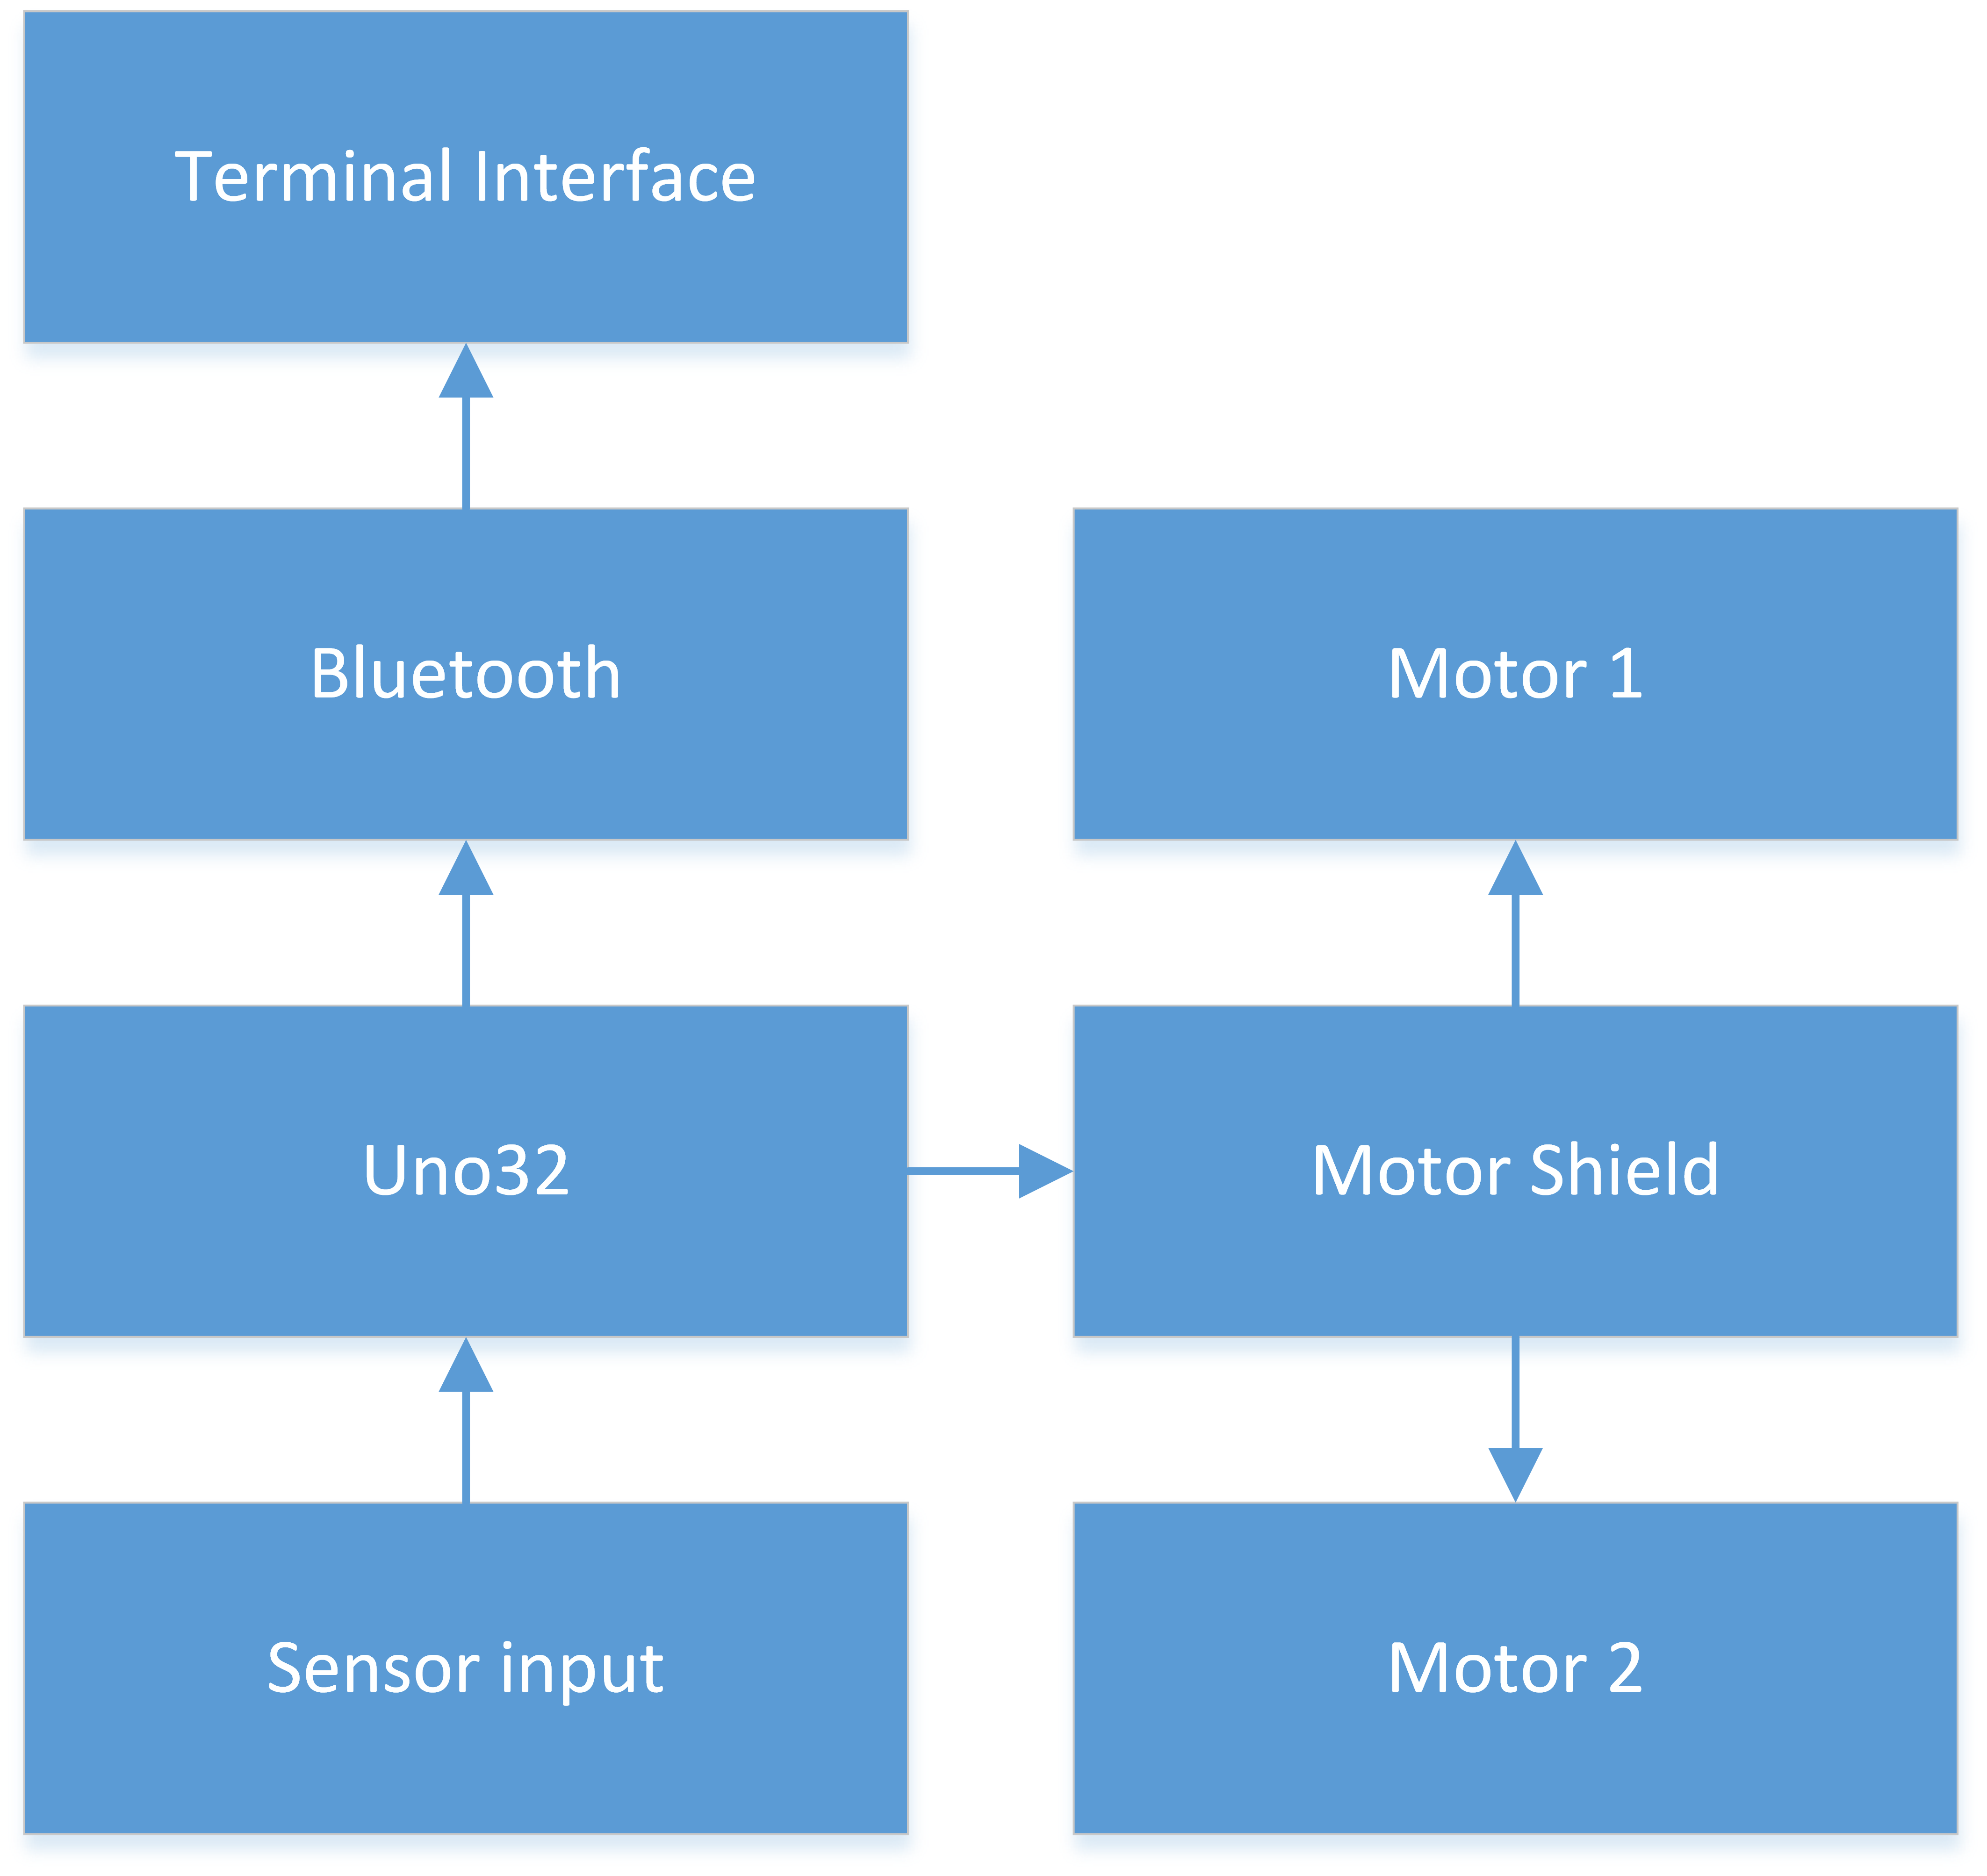
\includegraphics[width=0.7\textwidth]{figures/UdklipDIA2.png}
	\caption{\text{Hardware diagram with arrows}}
	\label{Hardware diagram}
\end{figure}

The micro controller is connected to the motor-shield.\ The motor-shield is then connected to the two motors, called motor 1 and motor 2 and is powering both motors.\ The micro controller is receiving data from the sensor set; the ultrasound sensors and the tachometer sensor.\ The micro controller then receives the data from the sensors and sends it further to the Bluetooth transceiver and then the Bluetooth transceiver will send it to the interface. \\ \\

\section{Sensors and sensor concept}
The robot will utilize 3 ultrasound sensors. These will be working together to make the robot able to navigate open spaces more precisely. The 3 sensors are able to cover blind spots for each other and in this way provide for a more solid solution to object avoidance. They are mounted in a way such that there is one facing forwards, and one pointing out sideways from these, in a roughly 90 degree angle. This works for the robot in multiple ways; it covers blind spots and also allows the robot to "see" to its sides while moving straight forwards, this allows for more fluid object avoidance, since the robot can cut down on the amount of turns it has to make to follow an object to its side.

\subsection{Choice of sensors}
To find out what ultrasound sensors to use in navigating the robot, two sensors were compared briefly on their specifications; The HC-SR04 and the PING))) Ultrasonic Distance Sensor.\\
The specifications have been put into a table for a quick perspective into the sensing distance, volt, current and price for each sensor.\\

As seen on the table; the two sensors with slight differences, the HC-SR04 can measure an extra meter compared the PING)). Additionally, there's a staggering price difference of approximately 200,- DKK between the HR-SR04 and the PING))), which is a concerning factor when producing multiple robots.\\

In the case of this project, the device available is the HC-SR04. Even if the PING))) was available, the HC-SR04 has 4 pins compared to the PING))) with only 3 pins, this feature can make it easier to manage when coding the sensor.\\

\begin{table}[!ht]
\centering

\label{Sensor table}
\begin{tabular}{|l|l|l|}
\hline
\textbf{Name}           & HC-SR04   & PING)))    \\ \hline
Max/min sensor distance & 4m-2cm    & 3m-2cm     \\ \hline
Working current         & 15mA      & 30mA       \\ \hline
Voltage                 & 5DC       & 5DC        \\ \hline
Price                   & 17.63,- DKK & 211.53,- DKK \\ \hline
\end{tabular}
\caption{Sensor table \cite{HC-SR04} \cite{PING}}

\end{table}

Even if availability wasn't a limitation, the clear choice would be the HC-SR04, due to the more impressive range and the better pricing of the HC-SR04.

\subsection{Ultrasound sensor - HC-SR04}
When a robot should be able avoid obstacles it will need a device to inform the robot where it's position is compared to the obstacle. This is where an ultrasound sensor plays an important role. For this task the HC-SR04 has been picked.\\

\begin{figure}[!ht]
	\centering
	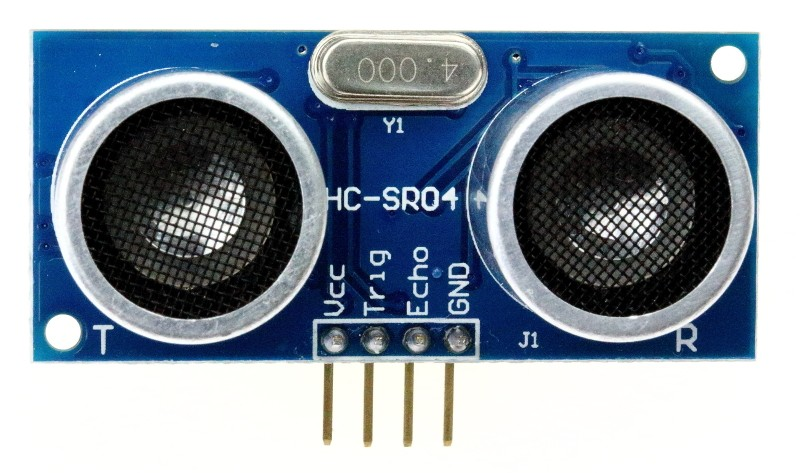
\includegraphics[width=0.7\textwidth]{figures/hc04.jpg}
	\caption{\text{The HC-SR04 ultrasound sensor}}
	\label{HC-SR04}
\end{figure}


The way the ultrasound sensor works is by emitting acoustic waves and then waits for the waves to reflect back to the sensor. The waves are often at about 40 kHz and humans are unable to detect the sounds because of the frequencies being above the human audible range.\

What is causing the device to make ultrasonic sound is a piezoelectric crystal. The crystal is receiving a rapid oscillating electrical signal, this causes the crystal to expand and contract and thereby creating a sound wave.\ The sound waves will then after being reflected return to a piezoelectric receiver which can then convert the waves into voltage by using the same method as explained above. \\

There are several popular ways to process the information gathered from the ultrasound sensor.\
\begin{enumerate}
	\item[•]Time of flight
	\item[•]Doppler shift
	\item[•]Amplitude attenuation
\end{enumerate}

In the scope of the project, the robot will be using "Time of flight" for sensing the distance between itself and the obstacle.\

When working with the term time of flight, it means the ultrasound sensor only generates pulses of sound instead of an continuous streak of sound waves. to avoid confusion. In high speed situations this will mean there is waiting time limits.\\ 

The calculation for using the ultrasound sensor is:\\

t = time\\
r = distance travelled\\
c = speed of light\\

r= c*t\\

With this the robot can calculate the time of flight.\

\subsubsection{Considerations:}
When using the ultrasound as a sensing tool, there are some factors that must be taken into consideration.\\ Temperature and humidity can affect the speed of sound, just as air currents have been known to be able to create invisible boundaries that can reflect ultrasonic waves.\\
Ultrasound sensors have something called a dead zone, this occurs when an object is in front of the sensors and the receiver can't keep up.\\
Some materials are very absorbent, which will result in less reflected ultrasound to be detected by the receiver.

\subsubsection{Mounting}

For putting the sensors in place facing the right directions, a 3D-printed mount was made and then bolted to the chassis of the bot. 

\begin{figure}[!ht]
	\centering
	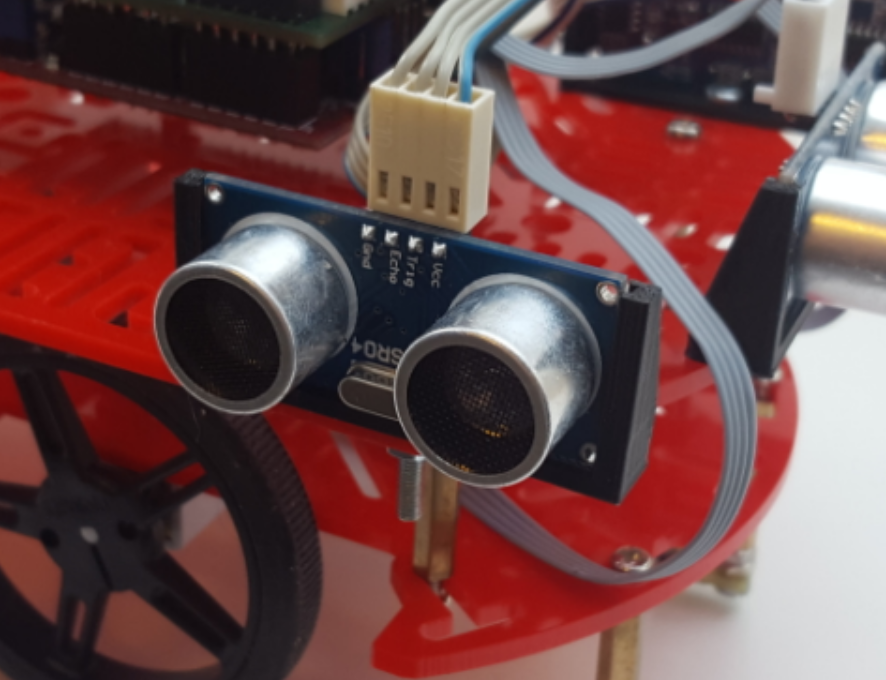
\includegraphics[width=0.7\textwidth]{figures/Mount1.png}
	\caption{\text[Sensor mount]{Mounts made by 3D printing, for ultrasound sensors}}
	\label{Mount}
\end{figure}

%\subsection{Infrared sensor - QRE1113}

%The robot will make use of infrared sensors in symbiosis with the aforementioned ultrasound sensors.\\ This will %allow it to take readings on a wider array of surfaces, as infrared sensors are better suited for less even %surfaces.\\ They work by emitting infrared light onto a surface, and then taking a reading based on the amount of %light that gets reflected. A light surface will reflect more light back than a dark one.\\ The sensor will then %output a feedback signal made of a certain amount of voltage, ranging from 1\% to 100\%, based on how much light %was reflected back. Based on this output voltage, it is possible to use an ADC to convert these signals into %digital signals, which can be monitored more conveniently.\\ Functionally, the robot is left with a way of %knowing which surface the sensors are above - and in the case of a track with a black line to follow, this allows %it to detect where the line it needs to follow is.\\

%Due to past experiences, the QRE1113 sensor has been chosen to be utilized on the robot to enable its line-f%ollowing properties and positioning

%\begin{figure}[!ht]
%	\centering
%	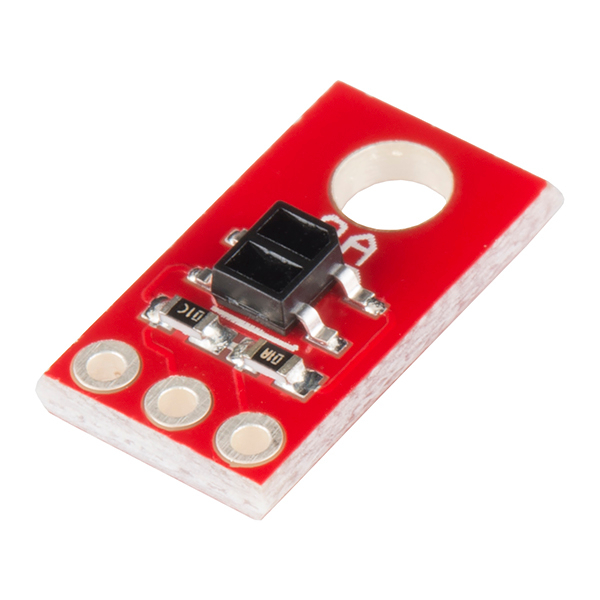
\includegraphics[width=0.7\textwidth]{figures/QRE.jpg}
%	\caption{\text{Mounted QRE1113 sensor}}
%	\label{Hardware diagram}
%\end{figure}

\section{The chipKIT Uno32 board}\fixme{section need readover}
The robot will utilize the chipKIT Uno 32 board to execute code. The board
was chosen both due to past experiences, but also because the robot would need
line-following properties, and we had already written a functional line-following robot
previously, which also included some important features, including PID control and 
pulse-width modulation patterns. \\
This enabled a lot of recycled code, which was a strong point
in the Uno 32's favor due to time constraints. \\

The board is also compatible with Arduino shields, and as such designing the H-bridge for it
becomes more straightforward. It's fast enough to execute the code, and works well within the
input power the robot will utilize.

\section{The motor shield}
The motor shield is the single add on board used in the project, and contains all the features needed for making the robot work.
The features are:
\begin{enumerate}
	\item[•]Dual H-bridges.
	\item[•]Low side current sensor for each H-bridge.
	\item[•]CPLD for reconfigurable H-bridge logic control.
	\item[•]All connectors needed for sensors and other units needed:
	\begin{enumerate}
		\item[•]Screw terminal for motor connection.
		\item[•]Screw terminal for input power.
		\item[•]Molex connector for ultrasound distance Sensor.
		\item[•]Molex connector for  distance sensor.
		\item[•]Molex connector for motor encoder.
		\item[•]Molex connector for infrared light sensor.
		\item[•]Header for Bluetooth module.
	\end{enumerate}
\end{enumerate}

\begin{figure}[!ht]
	\centering
	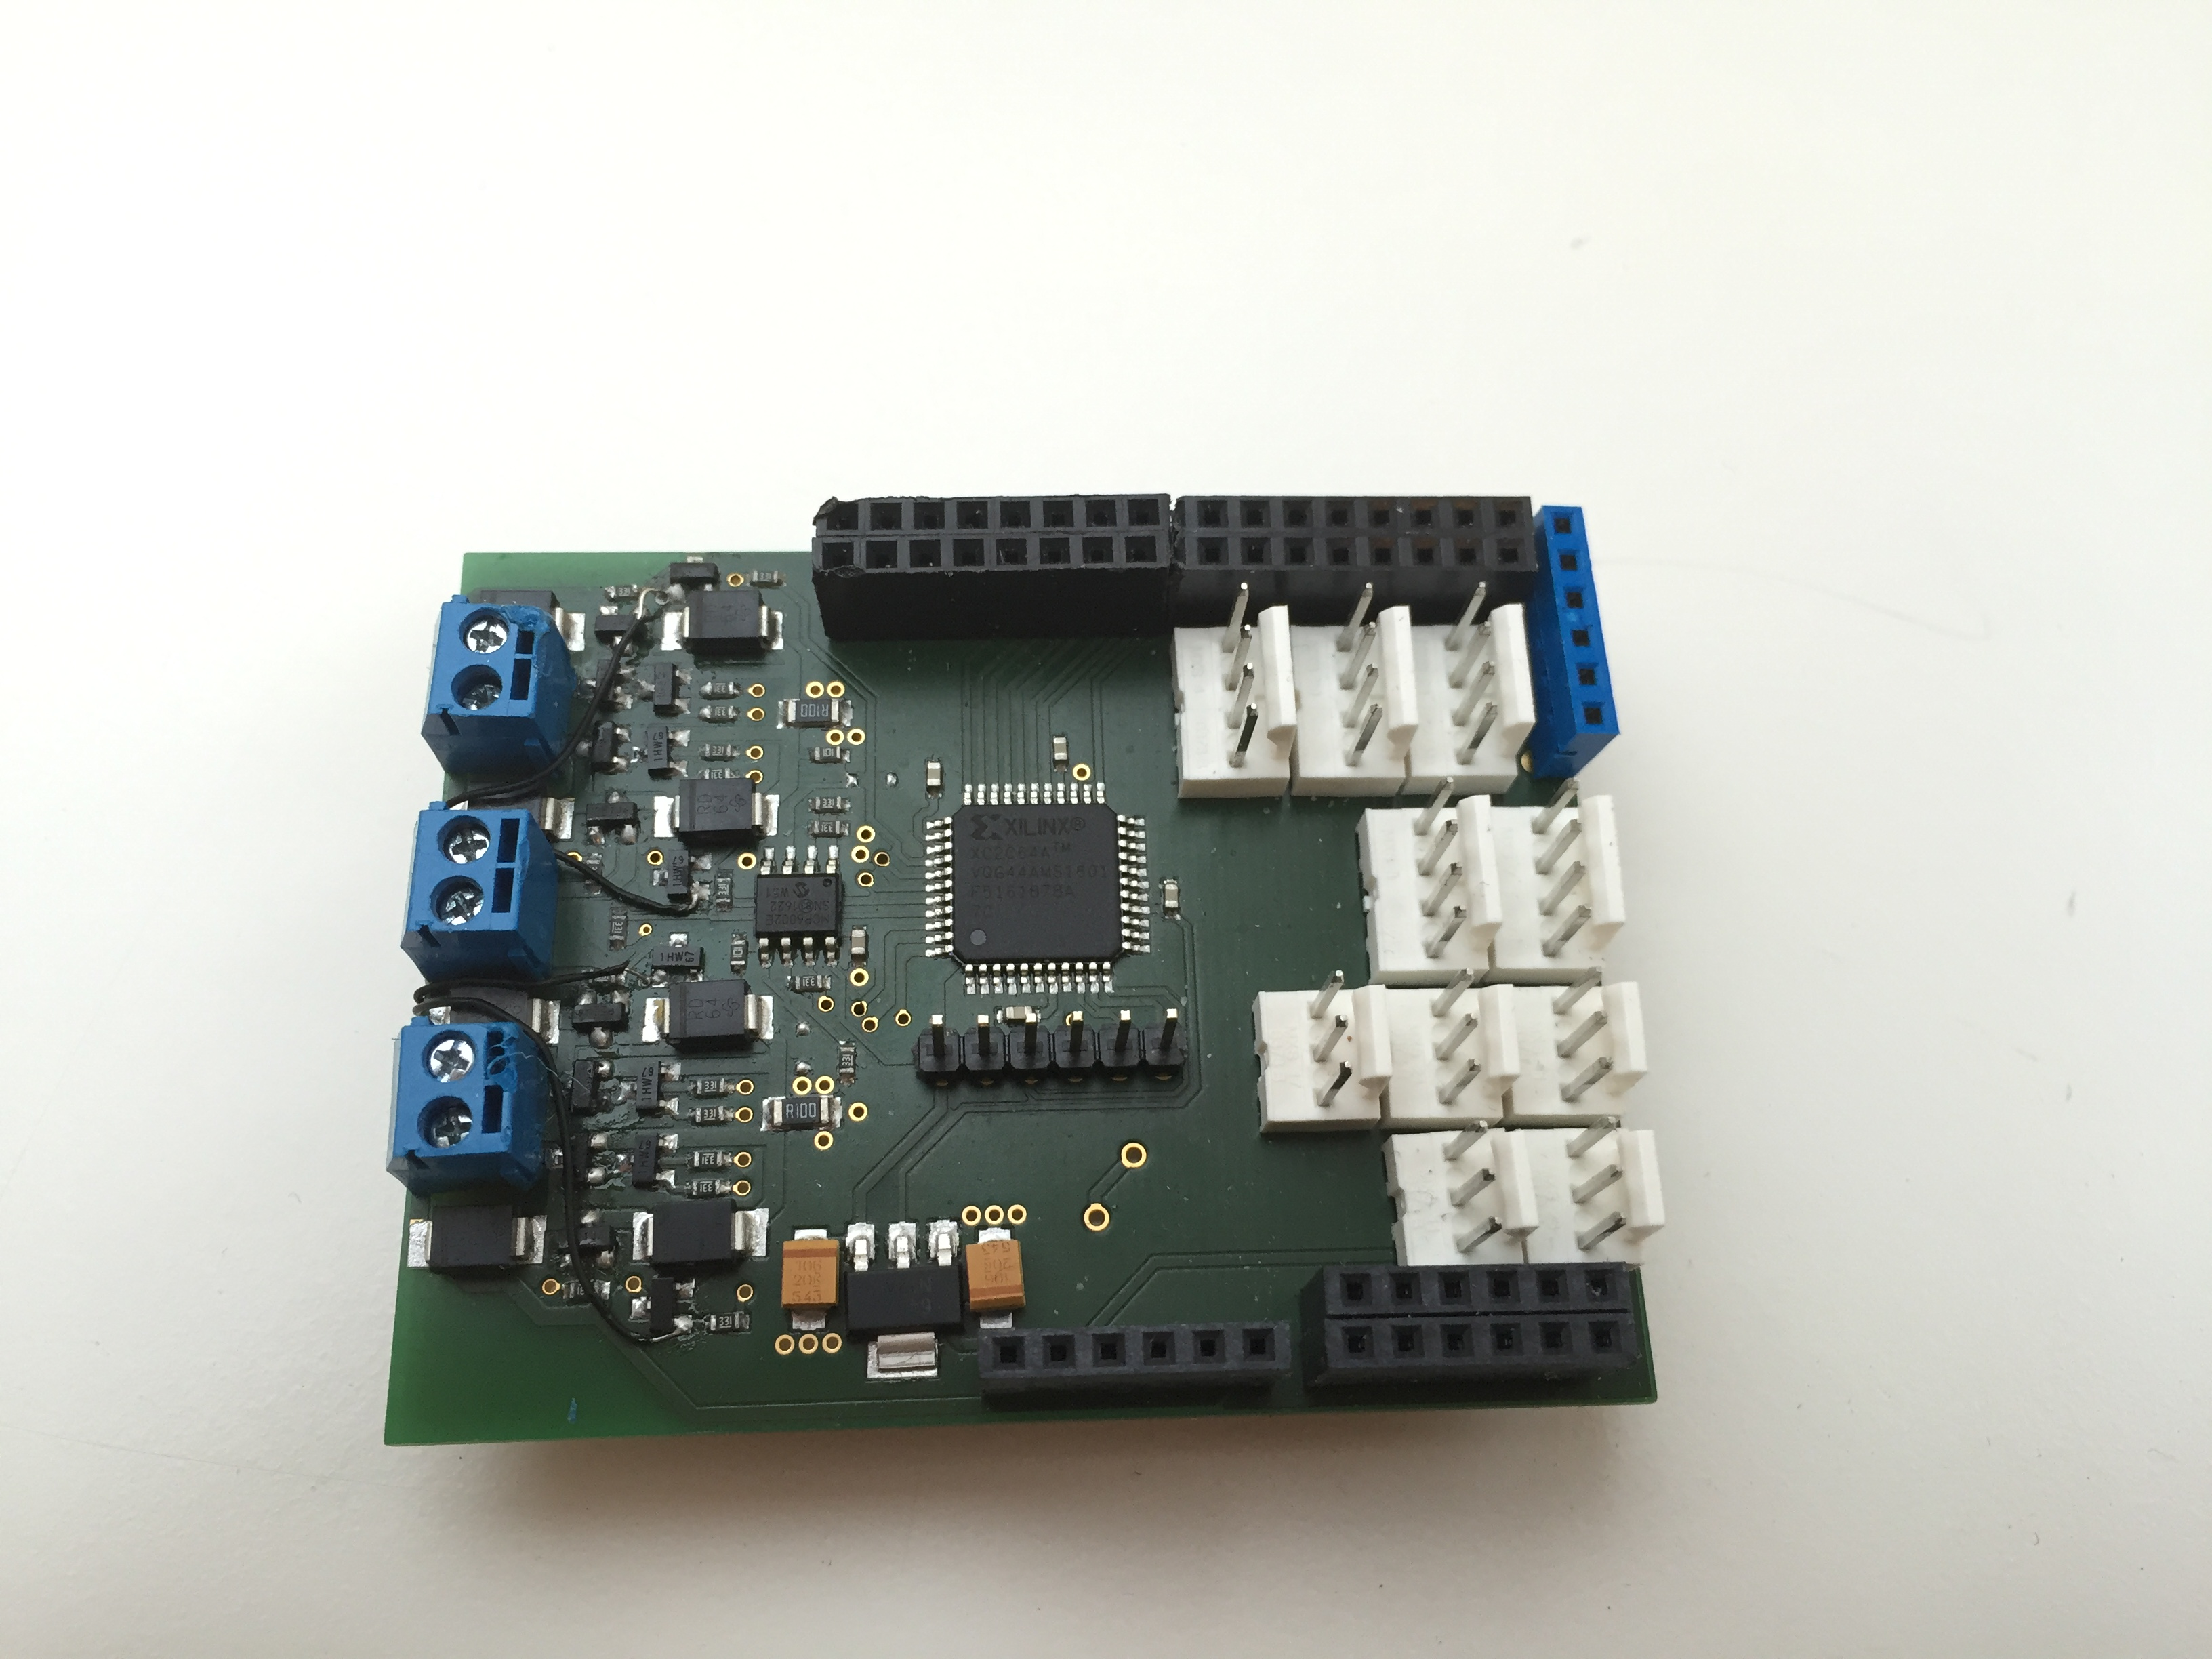
\includegraphics[width=0.7\textwidth]{figures/motorShield.jpg}
	\caption{\text{The self-designed motor-shield}}
	\label{Motorshield}
\end{figure}

\subsection{The H bridge}
The robot will make use of an H-bridge. An H-bridge is a circuit made for controlling the motor of the robot, by making sure the motor will never try to do forward and backward motion  and cause errors or short circuits. The point of using an H-bridge is to ensure motor safety and functionality.

\subsection{Pololu 100:1 Micro Metal Gearmotor 6V High Power}

This is a small motor, drawing 120mA when there is no load, and 1600mA when stalling. They run up to 320 RPM; because of this, the robot will be able to move very rapidly. The ones used for the robot have an extended motor shaft, which makes it possible to utilize the Pololu motor encoders.

\begin{figure}[!ht]
	\centering
	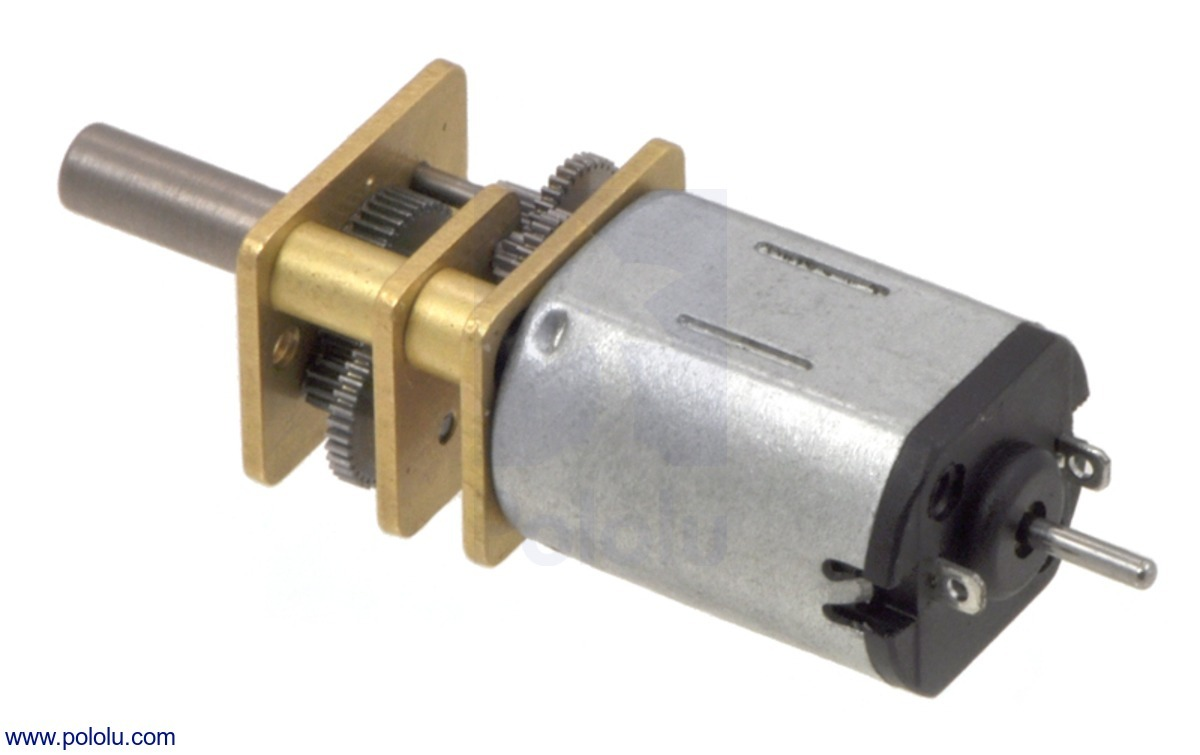
\includegraphics[width=0.7\textwidth]{figures/pololu.jpg}
	\caption{\text{Pololu micro metal gear motors}}
	\label{Hardware diagram}
\end{figure}

\subsubsection{Pololu Magnetic Encoder Pair Kit}

These encoders allow the transmission of data based on motor movement. It works by having the encoder board count the revolutions of the magnetic disc mounted on the board. It does this twelve times per revolution. The transmission of this data allows the robot to monitor how long it has traveled. This data, along with directional data coming from the code, will allow the robot to track its own movement in a coordinate system. This way, the robot will always start on (0, 0), and if given a destination coordinate to navigate towards, it will be able to both find the most efficient way there, but also track its movement throughout the runtime.

\begin{figure}[!ht]
	\centering
	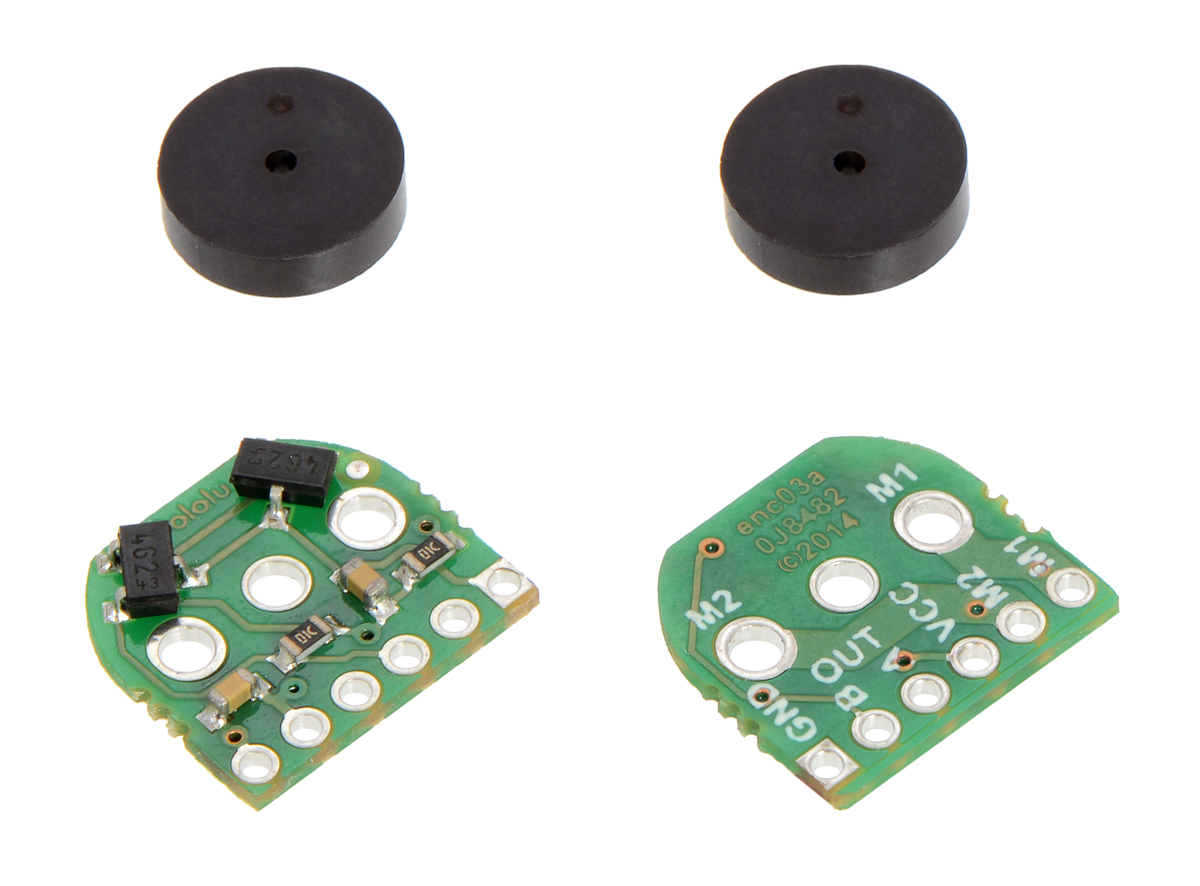
\includegraphics[width=0.7\textwidth]{figures/pololuEncoder.jpg}
	\caption{\text{Pololu Magnetic Encoder Pair Kit}}
	\label{Hardware diagram}
\end{figure}

\section{The Bluetooth tranceiver}
The robot will utilize the BlueSmiRF Silver bluetooth tranceiver. The transceiver is made by Sparkfun, it is utilized to make use of an GUI, by sending data from the MCU to the computer (GUI) by the use of bluetooth.\\ The bluetooth tranceiver makes it possible to monitor both the inputs and the logic behind the steering. The baudrate is between 2400-115200 bps and the tranceiver can be powered from 3.3v up to 6v. 

\section{Part conclusion}
After initial H-bridge problems, the rest of the process of building the robot went according to plan, and there were no future issues. The robot utillize a range of components which have been used for previous projects, which made the project much more simple to work with. This eliminated some of the learning curve that the previous robot presented, and made it possible to plan out and assemble the robot very rapidly, even though a lot of time was spent waiting for components for the motor shield, and the faulty components. This way, a lot more time could be used on programming and other software solutions. 
